\chapter*{\FontH{\Huge Die Insel der Grossen Krähe}}
\addcontentsline{toc}{chapter}{Die Insel der grossen Krähe}
\lettrine[lines=3]{\color{DeepPink}A}{ls} die Grosse Krähe die Menschen erschuf, lebten diese in einem Dorf auf einer Insel mitten im Meer. Das Meer wimmelte von Fischen; Obst und Gemüse wuchsen prächtig und ab und an liess sich auch ein Wildschwein fangen. Das waren dann immer besondere Tage. Die Menschen zogen ihre schönsten Kleider an und trafen sich auf dem Platz des einzigen Dorfes, machten Musik und sangen solange das Schwein über dem Feuer bruzelte.

Die Menschen achteten die Grosse Krähe und brachten ihr jede Woche kleine Geschenke. Das waren meistens Muscheln, die die Kinder am Strand gefunden hatten oder der Zahn eines Wildschweins oder auch eine besonders schöne Blume. Dafür beschützte die Krähe die Menschen und zeigte ihnen, wie das Feld bestellt wird und Häuser gebaut werden.

Die Grosse Krähe lebte auf dem höchsten Berg der Insel und dort auf dem höchsten Baum, ganz auf der Spitze. Von da konnte sie die ganze Insel überblicken. Wenn jemand Hilfe brauchte, kam sie geflogen und tröstete ihn. Und wenn jemand krank wurde, setzte sie sich so lange neben das Krankenbett, bis der Kranke wieder gesund war. Die Menschen liebten die Krähe dafür wie ihre Mütter.

Kanouk war einer der Dorfbewohner. Er war jung und geschickt und wurde von allen geachtet. Er konnte schneller laufen als alle anderen und interessierte sich für alles, was die Menschen damals kannten, was allerdings nicht sehr viel war. Am liebsten sass er am Strand und beobachtete die Vögel oder die Fische. Kanouk war der einzige, der wusste, wo sich die Wildschweine am Tag versteckt hielten. Aber das verriet er niemanden, denn er dachte, dass die Wildschweine alleine entscheiden sollen, wann sie gefangen werden wollten.

Einmal brach sich ein alter Mann auf der Suche nach Beeren im Wald ein Bein, als er über eine Wurzel stolperte. Kanouk hörte die Hilferufe und kam herbeigeeilt. Auch die Grosse Krähe kam und sagte, dass Kanouk nun nach Hause gehen könne. Sie werde bei dem verletzten Mann bleiben, so wie sie es immer getan hatte. Aber Kanouk hatte eine bessere Idee. Geschickt band er zwei starke Äste so zusammen, dass der alte Mann sich darauf legen und von Kanouk nach Hause gezogen werden konnte. Dort wurde er von seiner Töchtern versorgt, die ihn pflegten, bis das Bein wieder gesund war.

Die Grosse Krähe aber rief: 

\enquote{Ihr Menschen, ich habe Euch immer geholfen und war für Euch da. Ich habe Euch die Dinge gegeben, die ihr zum Leben braucht. Ich bitte euch nur um dies Eine: Seid zufrieden, mit dem was ihr habt. Strebt nicht nach immer mehr und immer besseren Dingen. Das führt nur zu Neid und Hass unter Euch und auch mich werdet ihr dann nicht mehr achten und brauchen. Wenn ihr nicht die Tradition wahrt, missachtet ihr eure Ahnen und  ich muss euch verlassen.} 

Die Menschen senkten die Köpfe und versprachen, nichts mehr selbst erfinden zu wollen. Sie schalten Kanouk, der die Trage für den alten Mann gebaut hatte und ihn ins Dorf zurück gebracht hatte. Er aber dachte, dass es doch nicht falsch sein kann, anderen Menschen zu helfen.

Das war ihm schon oft passiert. Einmal hatte er eine Rinne gegraben, damit das Wasser von der Quelle direkt ins Dorf geleitet wurde, ein anderes Mal hatte er Palmenwedel so zusammen gebunden, dass sich Kinder in sie hinein setzen und so die Dünen damit herab rutschen konnten. Jedes Mal war die Grosse Krähe geflogen gekommen und hatte seine Erfindungen verboten. Das ärgerte Kanouk, der anfing sich zu wünschen, an einem anderen Ort wohnen zu wollen. Überhaupt wünschte er sich nichts sehnlicher, als dass die Welt nicht nur aus der kleinen Insel bestehen würde, sondern noch mehr zu bieten hätte.

\afterpage{
    \begin{figure}
        \thispagestyle{empty}
        \centering
        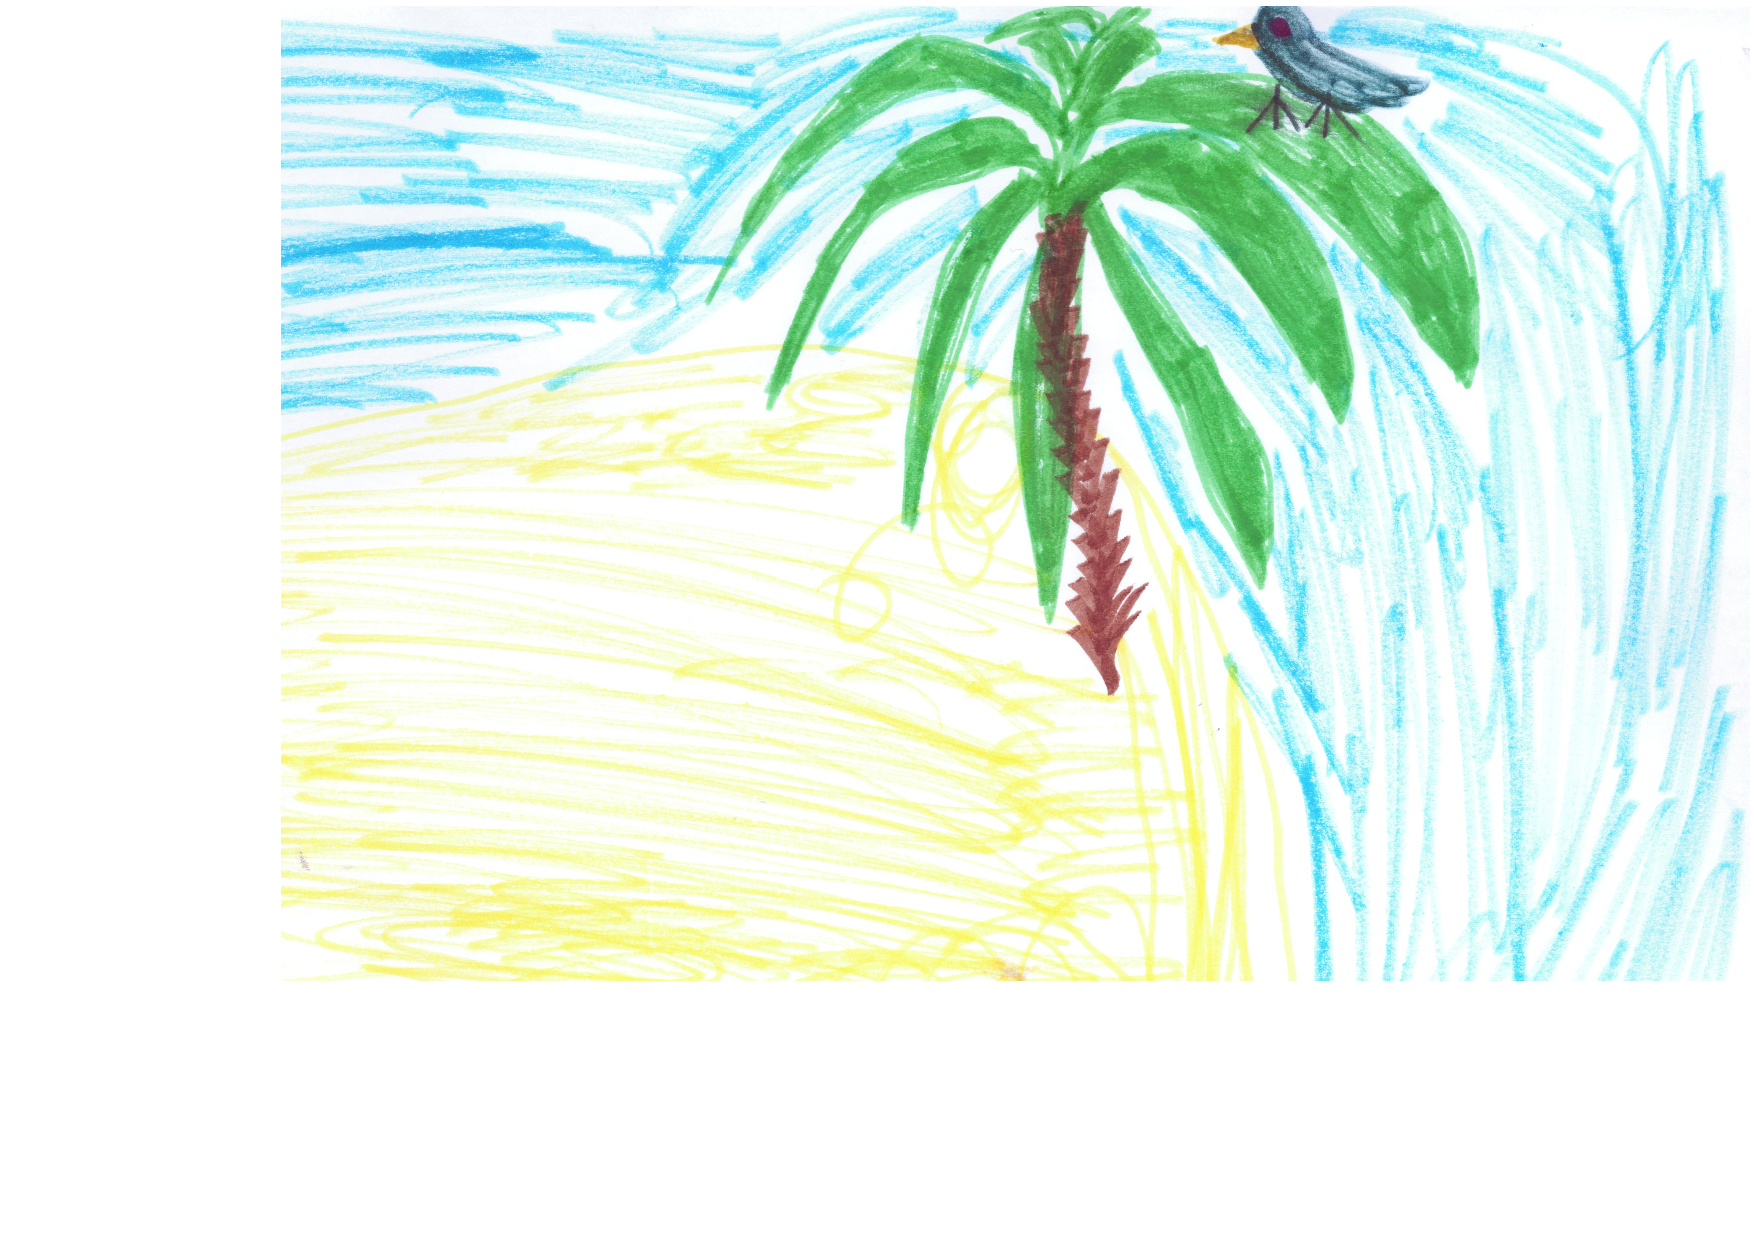
\includegraphics[width=\textwidth]{bilder/1kraehe.pdf}
    \end{figure}
    \clearpage
}


Auch wenn die Grosse Krähe ihm schon so viel verboten hatte, achtete Kanouk sie jedoch wegen ihrer Weisheit und ihres Wissens. Daher beschloss er, sie um Rat zu fragen. Sollte die Welt wirklich am Strand zu Ende sein, oder wussten die Fische vielleicht, ob es noch andere Inseln gäbe. Also machte sich Kanouk auf zur Grossen Krähe. Es dauerte einen Tag und fast die ganze Nacht, bis er den Berg erklommen hatte und den Baum der Grossen krähe erreichte. Der Baum war riesig und sehr alt. Zwischen den Ästen sass die Krähe und beobachte Kanouk sehr genau, als er seine Frage stellte. Nach einer langen Zeit des Überlegens antwortete sie:

\enquote{Ich weiss, warum du diese Frage stellst Kanouk.} Und während die Krähe sprach, wurde der Himmel immer dunkler, der Wind legte sich und kein Vogel war mehr zu hören. Die Grosse Krähe schien riesig zu sein, als ob sie die ganze Insel überdecken konnte. Oder war Kanouk nur sehr klein geworden? 

\enquote{Dich treibt es hinaus in die Welt. Was denkst du, was dich erwarten würde, wenn du andere Inseln findest? Meinst du, dass es dort anders ist als hier? Die Früchte süsser und die Fische grösser? Und zu welchem Preis? Andere werden dir folgen, das Dorf und damit unsere Tradition werden sterben. Das werde ich nicht zulassen! Ich werde dich aus der Gemeinschaft des Dorfes für immer ausstossen.} 

Plötzlich sah sie wieder sehr freundlich und mütterlich aus. Die Vögel zwitscherten wieder, der Wind blies und die Sonne schien.

\enquote{Natürlich gibt es keine anderen Inseln, was denkst du nur. Von hier oben sehe ich die ganze Welt, aber ich sehe nirgends am Horizont auch nur das kleinste Zeichen von Land. Komm zu mir herauf geklettert, dann zeige ich dir die ganze Welt.} Also kletterte Kanouk auf den Baum der Grossen Krähe und blickte sich um. Nichts, gar nichts so weit das Auge reichte. Die Grosse Krähe sprach weiter:

\enquote{Wie du siehst, da ist nichts, denn da kann nichts sein, ausser dem Meer. Bis zum Ende der Welt nur Wasser. Aber ich verspreche dir, wenn du aufhörst, so viele Fragen zu stellen und die fremden Inseln vergisst, lass ich dich immer einmal im Jahr auf meinen Baum klettern. Als einzigen im Dorf. Man wird dich achten und respektieren und du sollst der Chef des Dorfes werden.}

Traurig kehrte Kanouk in sein Dorf zurück. Er hatte seinen Plan aufgegeben. Nicht weil er Chef vom Dorf werden wollte, sondern weil er wirklich nichts gesehen hatte. Die Welt ist nur eine Insel mitten im Meer. Die nächsten Wochen verbrachte Kanouk alleine in seiner Hütte und dachte über das Angebot der Grossen Krähe nach, konnte sich aber den ganzen Sommer lang nicht entscheiden. Kanouk wusste jetzt, dass es keine anderen Inseln gab und das tat ihm weh.

Wie jeden Herbst kamen auch in diesem Jahr die Stürme. Gewöhnlich waren die nicht sehr stark, nur hin und wieder wurden ein paar Palmenwedel weggeblasen, mit denen die Menschen ihre Dächer bedeckten. Dieser eine Sturm war etwas schlimmer und er hielt viel länger an als sonst. Der Wind wollte für fünf Tage und fünf Nächte nicht aufhören zu blasen. Die Menschen verliessen ihre Häuser und suchten Schutz in einer Höhle. Als der Sturm sich endlich wieder gelegt hatte, kehrten sie in ihr Dorf zurück und sahen, was der Wind angerichtet hatte. Viele Dächer waren abgedeckt, aber das war nicht schlimm, das konnte schnell repariert werden. 

Aber es war noch etwas anderes geschehen. Hier und da sassen kleine Tiere, wie sie die Menschen bis dahin noch nicht gesehen hatten. Und weil sie die Tiere vor allem auf trockenen Palmwedeln fanden und sie so schrecklich aussahen, nannten sie sie Heuschrecken. 

\enquote{Das ist kein gutes Zeichen}, riefen sie, \enquote{Wir haben bestimmt die Grosse Krähe verärgert.} So überlegten alle, was sie wohl zu bedeuten hätten, aber da die Heuschrecken nach ein paar Tagen alle samt von den Vögeln gefressen wurden, gerieten sie bald in Vergessenheit. Nur Kanouk konnte sie nicht vergessen. Ihn quälte die Frage, wo die Heuschrecken wohl hergekommen waren. Hatte sie der Wind geboren? Das konnte er sich nicht vorstellen. Alle Tiere hatten Vater und Mutter, soweit er das beobachten konnte. 

Nachdem er sehr lange über die Frage nachgedacht hatte, rief er das Dorf zusammen und verkündete:

\enquote{Meine Freunde, ich habe lange überlegt, wo die Heuschrecken wohl hergekommen sind. Ich glaube der Wind hat sie zu uns geweht, denn ihr wisst, sie waren erst nach dem schlimmen Sturm hier. Aber aus dem Wasser kommen sie nicht, denn sie sehen aus, wie unsere Käfer, sie müssen von einer anderen Insel sein.}

Da fingen die anderen Dorfbewohner an zu lachen.

\enquote{Von einer anderen Insel?}, riefen sie. \enquote{Schau dich doch um. Du selbst hast es gesehen und uns erzählt. Um uns gibt es nur noch Wasser. Die Grosse Krähe hat nur das Meer und unsere eine Insel erschaffen, dahinter kommt nichts mehr. Und jetzt lass uns in Ruhe mit deinen dummen Ideen. Du verärgerst die Grosse Krähe und dann sind wir alle verloren.}

Kanouk konnte jetzt an nichts anderes mehr denken, als an die Frage, wie er wohl über das Wasser käme. Er war sich sich wieder sicher, dass es irgendwo noch Land geben muss. Gewiss, er war ein guter Schwimmer, aber das Meer war viel zu gross. Da half ihm der Zufall. Als er eines Nachmittags am Strand sass, fiel gerade vor ihm eine Kokusnuss ins Wasser und trieb mit den Wellen davon. Das war die Lösung. Er musste nur etwas bauen, dass wie eine Kokusnuss schwimmt, aber gross genug, dass er darin Platz hatte!

Kanouk fing an, vieles auszuprobieren, die Leute wunderten sich immer mehr und wurden immer wütender auf ihn. Die Angst vor der Grossen Krähe war einfach zu gross. Aber Kanouk hatte keine Zeit sich um solche Sorgen zu kümmern. Er warf grosse Steine ins Wasser und bastelte riesige Schalen aus Palmenwedeln, die er auch ins Wasser setzte, bis sie untergingen. Eines Tages rannte er durch das Dorf und rief schreiend 

\enquote{Ich hab's, ich hab's!}

Verwundert lief das Dorf zu der Stelle am Strand, wo Kanouk in letzter Zeit gesessen und gebastelt hatte. Etwas, dass ein wenig aussah wie eine Schüssel lag mit der Öffnung nach oben im Sand. Sie war aus dem Holz der Palmen gemacht und mit dem Harz der Nadelbäume gestrichen. 

\enquote{Was soll das denn sein?} fragten sie sich und kratzen sich am Kopf. 

\enquote{Ich nenne es Boot,} sagte Kanouk, \enquote{Und ich werde damit über das Meer reisen!}. Da wurden die Dorfbewohner zum ersten Mal richtig neugierig. Es stimmte ja, was Kanouk gesagt hatte. Irgendwo mussten die Heuschrecken hergekommen sein. Da kam die Grosse Krähe geflogen und rief mit donnernder Stimme:

\enquote{Ihr Menschen, ich hatte Euch gewarnt. Ihr sollt nicht Dinge bauen, die ich Euch nicht gezeigt habe. Ich weiss, dass Kanouk dieses Ding alleine gemacht hat. Deswegen will ich nur ihn bestrafen. Kanouk, Du bist ausgeschlossen aus unserer Gemeinschaft und sollst nie wieder in unser Dorf zurückkehren. Und wenn jemand von Euch Menschen auf seiner Seite ist, soll er es jetzt sagen.}

Die Menschen erschraken, senkten die Köpfe und liefen ins Dorf zurück. Kanouk blieb alleine am Strand zurück. Er ja nichts mehr zu verlieren, also nahm er seine Angel und so viele Lebensmittel, wie er finden konnte, steckte alles in sein Boot und stiess es hinaus ins Meer. Er sprang hinein und tatsächlich. Das Boot schwamm und er mit ihm. Noch nie im Leben war Kanouk so aufgeregt wie in diesem Augenblick. Die Strömung erfasste ihn und langsam trieb er vom Strand weg in die offene See. Wind wehte ihm durch die Haare. Die Palmen am Strand wurden aus der Ferne immer kleiner. Und so trieb Kanouk davon, um nie wieder auf seine Insel zurückzukehren.

Viele Tage lang sah Kanouk nur Wasser, so weit er blicken konnte. Er bekam Angst. Gegen den Hunger konnte er fischen, trinken konnte er das Wasser des Regens. Als er schon glaubte, nie wieder Land sehen zu werden sah Kanouk eine Möwe. Und da wusste er, dass er bald Land finden würde. So wurde Kanouk der erste Mensch, der das Festland erreichte.

Die Menschen in dem Dorf aber konnten Kanouk nicht vergessen. Was war wohl aus ihm geworden? Und wer half jetzt, wenn sich jemand verletzt hatte. Nur der Trost der Krähe machte niemanden gesund, dass merkten die Menschen jetzt. Und eines Tages fassten sie allen Mut zusammen, den sie hatten und vertrieben die Krähe. Sie begannen, gemeinsam ein Boot zu bauen, damit sie hinaus fahren konnte aufs Meer, um Kanouk zu suchen. \hfill {\color{DeepPink}\decofourleft}
